\section{Abstract}\label{abstract}

Episodic memories are not veridical records of our lives, but rather are
better described as organized summaries of experience. Theories and
empirical research suggest that shifts in perceptual, temporal and
semantic information lead to a chunking of our continuous experiences
into segments, or `events'. However, the consequences of these
contextual shifts on memory formation and organization remains unclear.
In a series of three behavioral studies, we introduced context shifts
(or `event boundaries') between trains of stimuli and then examined the
influence of the boundaries on several measures of associative memory.
In Experiment 1, we found that perceptual event boundaries strengthened
associative binding of item-context pairings present at event
boundaries. In Experiment 2, we observed reduced temporal order memory
for items encoded in distinct events relative to items encoded within
the same event, and a trade-off between the speed of processing at
boundaries, and temporal order memory for items that flanked those
boundaries. Finally, in Experiment 3 we found that event organization
imprinted structure on the order in which items were freely recalled.
These results provide insight into how boundary- and event-related
organizational processes during encoding shape subsequent
representations of events in episodic memory.

\section{General Introduction}\label{general-introduction}

Although our experiences unfold in a forward and continuous manner, our
memories for those experiences are structured and organized around
specific events. For example, imagine spending a night out in New York
City. You might go out to dinner with friends, stop at a bar for a
cocktail, and then proceed to an evening concert. Prior research
suggests that in memory, the details of experience within a specific
event (i.e.~dinner, bar, or concert) are more tightly linked together
than details experienced in distinct events
\autocites{ezzyat_what_2011}{dubrow_influence_2013}. One explanation for
this finding is that episodic memories may contain information about
their unique contextual characteristics, such as their temporal and
spatial contexts, which could serve to bind a temporally extended
experience into a single episode \autocite{tulving_organization_1995}.
Thus, the contents of a memory may be structured and grouped by the
context in which the experience occurred. However, it remains unclear
how shared context among items (referred to here as `events') and
changes in context (referred to here as `event boundaries') influence
episodic memory representations, as well as mnemonic relationships
between episodes. In this series of studies, we investigated the
consequences of event boundaries during encoding on the organization of
long-term episodic memories by measuring several forms of associative
memory.

A large body of evidence supports the idea that organizational processes
engaged at encoding modulate the structure of our memories for those
experiences
\autocites{atkinson_control_1971}{farrell_temporal_2012}{lee_item_1981}{murdock_distributed_1983}{raaijmakers_search_1981}.
One computational account for how this occurs suggests that the contents
of our experiences are maintained in a limited-capacity buffer during
encoding \autocites{lehman_global_2009}{lehman_buffer_2013}. Item and
context representations that co-occupy the buffer become associatively
bound. When those maintained representations are no longer of use to the
participants, a `compartmentalization' operation is thought to clear the
contents of the buffer. Thus, bound episodic `events' could be a
downstream consequence of encoding-related organizational processes that
compartmentalize information through a selective integration mechanism.

Another conceptually related framework called Event Segmentation Theory
(EST) has formalized the idea that `segmentation' processes parse
ongoing experience into events and serve to guide efficient allocation
of cognitive processing resources in the moment
\autocites{reynolds_computational_2007}{zacks_event_2007}. This model
proposes that incoming perceptual information and prior experience are
actively integrated in working memory to generate predictions about what
is likely to occur in the near future. At event boundaries, when future
input may be unpredictable or `surprising', attention is drawn to novel
perceptual features in the environment and integration processes are
halted. Prior behavioral and neuroimaging results support the notion
that people are sensitive to event boundaries
\autocites{radvansky_across_2012}{speer_temporal_2005}{zacks_event_2007}{swallow_event_2009}{zacks_human_2001}
and that memory for information at boundaries is enhanced
\autocites{boltz_temporal_1992}{newtson_perceptual_1976}{schwan_cognitive_2004}.

While somewhat different in their implementation, both of these models
make the unique and interesting prediction that shifts in context may
lead to enhanced memory for boundary information at the expense of
ongoing integration processes. Put another way, while event boundaries
may lead to a memory enhancement for information encountered at the
contextual shift, they may in fact have a detrimental effect on
relational memory for pairs of items that flank that boundary due to an
interruption of ongoing maintenance/integration processes. Prior
research has typically focused on the positive effects of This series of
experiments was designed to test the idea that contextual shifts may be
good for `in-the-moment' (within-trial) memory encoding at the expense
of across-trial associative encoding.

First, we predicted that items encountered at event boundaries would be
more tightly bound to their context, as attention may be shifted away
from the maintenance of previous `within-event' information to the
changing contextual features in the environment. While previous studies
suggest that that item memory at boundaries may be boosted
\autocites{boltz_temporal_1992}{newtson_perceptual_1976}{schwan_cognitive_2004},
here we explore specifically whether item are more tightly bound to
their associated contexts at event boundaries. We addressed this
question in our first experiment.

Second, we predicted that integration processes that may occur among
contiguous items that share a perceptual context (i.e.~an `event') could
result in strengthened associative binding among those items relative to
pairs of items that were encountered in neighboring events. Put another
way, while event boundaries may lead to a memory enhancement for
information encountered at the contextual shift, they may in fact have a
detrimental effect on relational memory for pairs of items that flank
that boundary due to an interruption of ongoing item-item integration
processes. Recent work using narrative cued recall
\autocite{ezzyat_what_2011}, recency discrimination for sequences of
visual images \autocite{dubrow_influence_2013}, and temporal proximity
judgments \autocite{ezzyat_similarity_2014} is consistent with this
prediction, showing that several measures of associative memory reduced
for pairs stimuli that flank an event boundary (compared to items within
the same event). Finally (and critically), we predicted a trade-off
between item-context processing at event boundaries and across-event
integration processes, such that a stronger boundary effect may result
in worse across-event integration. We hypothesized that at boundaries,
attentional resources are redirected from the integration/maintenance of
previous within-event representations to changing features in the
environment. In other words, the subjective strength of the event
boundary to the participant should influence associative memory for
pairs of items studied across that boundary, such that a `larger'
boundary should result in worse across event associative memory.

The present set of experiments was designed to test these predictions by
assessing multiple forms of associative memory. In each of these
experiments, participants encoded lists of object stimuli that were
grouped into smaller mini-lists (i.e.~events) by a shared background
color. This simple perceptual manipulation of the background color
allowed us to ask whether low-level perceptual shifts in context have
consequences for later memory. In Experiment 1, we tested whether items
at perceptual event boundaries are more strongly bound to their context
(i.e.~the color background), relative to trials where there was no
contextual shift. In Experiment 2, we tested whether event structuring
led to reduced binding between items encountered in distinct events
vs.~within events, and also whether the speed of processing at
boundaries is related to the cost in across-event associative memory for
pairs of items. Finally, in Experiment 3 we utilize a more naturalistic
retrieval task (a free recall paradigm) to ask whether and how recall
behavior is organized according to the event structure of the
experiment.

\section{Experiment 1: Perceptual boundaries facilitate object-color
associative
memory.}\label{experiment-1-perceptual-boundaries-facilitate-object-color-associative-memory.}

\subsection{Introduction}\label{introduction}

In Experiment 1, we sought to understand how perceptual boundaries
influence associative memory for the local information presented at
boundaries. Participants encoded lists of objects that were embedded in
a colored frame (Figure 1). On each trial, they were instructed to
imagine the displayed object in the color of the background frame and to
make a pleasant/unpleasant judgment on the object-color combination.
Importantly, the color of the frame did not change for six consecutive
trials before switching to a new background color. We operationalized an
`event' as consecutive trials where the color of the frame stayed the
same. After each encoding list, participants performed an object-color
associative memory test. `Boundary' trials were defined as trials on
which the presented color frame was different from the previous trial;
`non-boundary' trials were all other trials (i.e.~the presented color
matched the color from the preceding trial). Boundary objects were
therefore objects that were encoded concurrently with a color frame
switch, while non-boundary objects were all other objects.

\begin{figure}
  \centering
  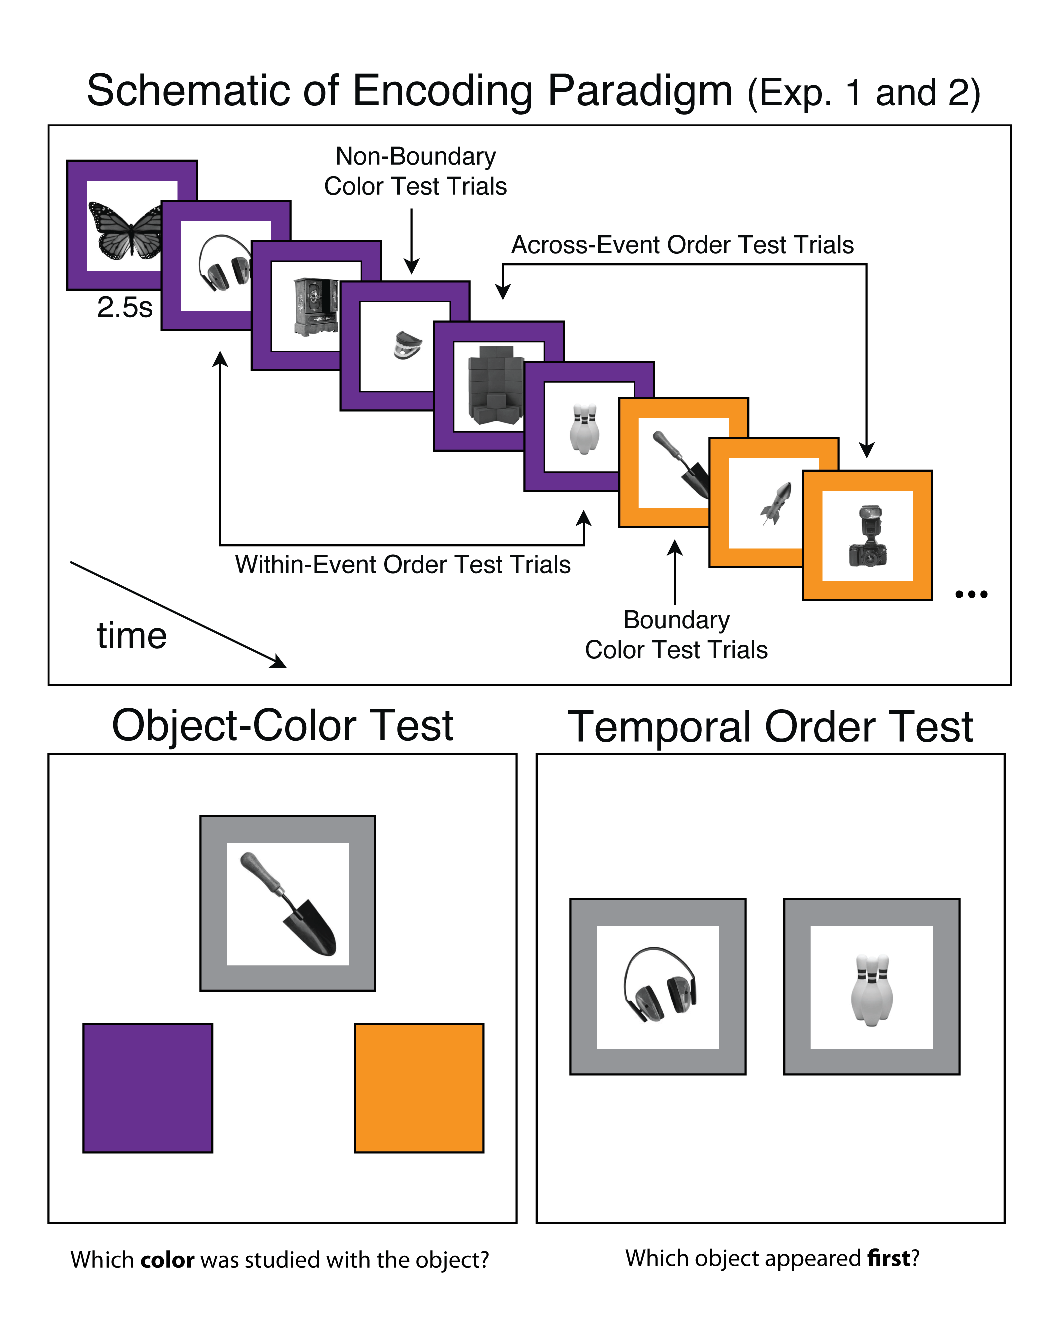
\includegraphics[width=.75\textwidth]{figures/chapter1_figure1.eps}
  \caption[Schematic of the Task]{\textit{Schematic of the Task.} Participants made pleasant/unpleasant judgments on object-color pairs.  Critically, the color switched every 6 trials. Object-color associative memory test. (Bottom, left)  After encoding, participants performed a two alternative forced choice object-color memory test. The object-color test was in both Experiment 1 and 2.  Temporal order memory test.  (Bottom, right) After the color test, temporal order memory was tested using a two alternative forced choice task.  Participants indicated which of two studied objects appeared first in the list. The temporal order test was only in Experiment 2.}
  \label{chapter1_figure1}
\end{figure}

The goal of Experiment 1 was to assess whether perceptual event
boundaries increased object-color associative memory. We predicted that
the memory enhancement would be specific to the boundary object-color
pair. A pattern of this nature would suggest a transient memory effect,
perhaps driven by a boundary-driven allocation of attentional resources
\autocite{kurby_segmentation_2008}.

\subsection{Methods}\label{methods}

\subsubsection{Participants}\label{participants}

Participants were 26 individuals (ages 18-35) recruited from New York
University and the greater New York Metropolitan Area. All participants
gave informed written consent in accordance with the University
Committee on Activities Involving Human Subjects (UCAIHS) and
participated in exchange for monetary compensation. We excluded
participants with chance memory performance (N = 2), leaving 24
participants for the statistical analyses. For all three experiments,
the sample size was chosen based on a power analysis (power = .8, alpha
= .05) of a separate study on boundary-related memory effects from
\textcite{dubrow_influence_2013}.

\subsubsection{Materials}\label{materials}

For all experiments, we used a stimulus set consisting of 576 gray-scale
pictures of objects from various online databases. A subset of these
stimuli was used for Experiment 1 (432 objects). Each one was resized to
a fixed size of 350x350 pixels. To generate colors for the frames, 24
unique colors were selected from color continuum ranging from
{[}0,0,0{]} to {[}255, 255, 255{]} RGB values. Lists of colors for each
block were generated, such that no two colors that occurred
consecutively at encoding could be perceptually similar. For example, if
the previous event color was red, the next color could not be orange,
but it could be blue or green. Furthermore, the same color could not
appear in a list more than once and colors were recycled after every
four lists. Stimulus order varied for each subject and stimulus-color
pairings were randomized across subject.

\subsubsection{Design and Procedure}\label{design-and-procedure}

Before the experiment began, there was a brief practice version of the
experiment to ensure that participants understood the task. For each of
12 study lists, participants intentionally encoded lists of 36
trial-unique gray-scale objects that were embedded on a colored frame.
Participants were instructed to imagine the object in the color of the
frame and decide if the object-color pair was pleasing. The participants
were instructed to respond as soon as they made a pleasantness decision
by pressing one of two buttons on the keyboard (`j' or `k'). The color
of the frame was identical for six consecutive objects before switching
to a new color for the next six objects. An `event' was defined as six
consecutive objects with the same colored frame. There were six events
per study list. On `boundary' trials, the frame color updated at trial
onset (i.e.~concurrently with the object). All other trials (event
positions 2-6) were called `non-boundary' trials. Objects were presented
for a fixed time of 2.5 seconds (s) with a fixed 2 s inter-trial
interval (ITI) followed by a .5 s fixation cross before the onset of the
next trial. The colored frame remained on the screen continuously during
the presentation of each event (including the 2 s ITI and a .5 s
fixation cross) and only changed concurrently with boundary objects. It
is important to note that the objects remained on the screen for a fixed
period of time (2.5 seconds). Thus, encoding response times in the rest
of this manuscript refer to the amount of time it took for the
participant to complete the pleasantness decision, not the duration that
the stimulus was on the screen.

Following each encoding list, we tested object-color associative memory.
To minimize recency memory effects, the test was structured such that
objects presented in the first half of the experiment (1:18) were tested
first and objects presented in the second half of the experiment (19:36)
were tested second. However, within each half, the test trials were
randomized. For each test trial, participants were shown a previously
studied object with a grey border presented above two colors that were
positioned on the left and right side of the computer screen (Figure 1).
One of these colors (target) was originally paired with the object while
the other color (lure) was always one of the colored frames that had
immediately preceded or followed the target color at encoding. The lure
was counterbalanced such that it was equally likely to precede or follow
the target color. Targets and lures were also equally likely to appear
in the left or right positions on screen. In one step, participants were
asked to indicate which of the two colors had been paired with the
object at encoding and also to indicate their confidence in their
decision (high/low confidence, HC/LC). Thus, there were a total of 4
possible responses during the test (HC left color, LC left color, HC,
right color, LC right color). Test trials were self-paced and advanced
as soon as a response was given, with a fixed .5 s ITI between test
trials. Half of the items in each encoding list were tested: We
alternated between testing of even (2:2:36) and odd (1:2:36) trials on
each list.

\subsection{Results}\label{results}

\begin{figure}
  \centering
  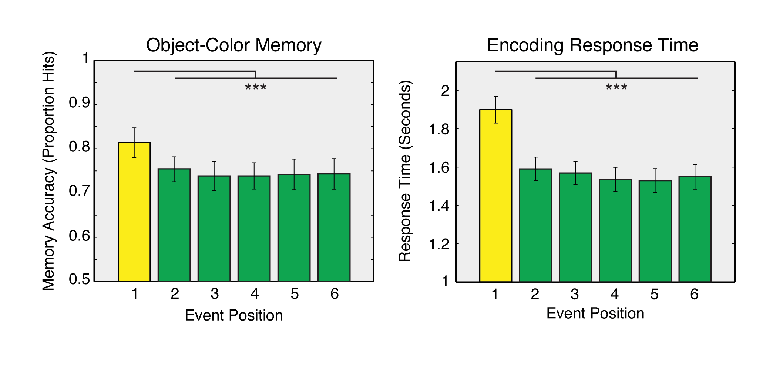
\includegraphics[width=.75\textwidth]{figures/chapter1_figure2.eps}
  \caption[Behavioral Experiment 1 Results]{\textit{Experiment 1 Results.} Object-color associative memory accuracy (left) and response times are shown as a function of within-event position (right).  The boundary condition is plotted in yellow and non-boundary conditions are plotted in green.  Error bars represent the standard error of the mean. *p<.05, **p<.005, ***p<.001.}
  \label{chapter1_figure2}
\end{figure}

\subsubsection{Effect of perceptual boundaries on color memory
performance.}\label{effect-of-perceptual-boundaries-on-color-memory-performance.}

We found that memory for the object-color association varied as a
function of event position {[}Figure 2; \emph{F}(5,115) = 5.23, \emph{p}
\textless{} .001, \(\eta^{2}\) = .185{]}. The position by confidence
interaction was not significant {[}\emph{F}(5,109) = .42, \emph{p}
\textgreater{} .1{]}, so we collapsed across high and low confidence
trials. A planned contrast revealed that color memory was significantly
better for the boundary condition compared to non-boundary conditions
{[}\emph{t}(23) = 5.54, \emph{p} \textless{} .001, Cohen's \emph{d} =
1.66{]} and follow up pairwise t-tests show that memory for the boundary
condition was significantly better than each non-boundary condition
{[}\emph{p}'s \textless{} .05{]}. Thus, object-color associative memory
at boundaries was significantly enhanced relative to trials that are not
studied at perceptual boundaries.

\subsubsection{Encoding Response times}\label{encoding-response-times}

Next, we asked whether perceptual boundaries also impacted RTs during
the successful retrieval of the object-color associations. We found that
RTs to correctly remembered trials varied as a function of event
position {[}\emph{F}(5,115) = 4.112, \emph{p} \textless{} .002,
\(\eta^{2}\) = .152{]}. The position by confidence interaction was not
significant, so we collapsed across confidence {[}\emph{F}(5,95) = 1.23,
\emph{p} \textgreater{} .1{]}. A planned contrast revealed that
retrieval of items from the boundary condition was significantly faster
than the non-boundary conditions {[}\emph{t}(23) = -3.01, \emph{p}=.006,
Cohen's \emph{d} = .88{]}. Subsequent pairwise t-tests revealed that
position 1 was significantly faster than positions 2, 4 and 6
{[}\emph{p}'s \textless{} .05{]}, and a trend for an effect for position
3 {[}\emph{p} = .059{]} and 5 {[}\emph{p} = .068{]}. Thus, during
retrieval, RTs to correct boundary trials were speeded relative to
non-boundary trials, suggesting that information studied at boundaries
is more accessible than non-boundary information.

\subsection{Discussion}\label{discussion}

Experiment 1 revealed that associative memory was enhanced for trials
that appeared at perceptual event boundaries. Prior studies that have
reported better overall memory for information studied at event
boundaries
\autocites{boltz_temporal_1992}{newtson_perceptual_1976}{schwan_cognitive_2004},
used clips from studied movies as retrieval cues and these cues taken
from event boundaries contained more diagnostic information about the
clips, which could ultimately account for the memory benefit. By
contrast, in the present study, the only difference between the boundary
and non-boundary conditions was a change in the color of the background
frame in the boundary condition. Therefore, during retrieval, the amount
of available perceptual information on each test trial was the same and
so, any differential effects we see in boundary memory must be related
to processes that occurred during encoding. Thus, the current finding is
consistent with these prior results but importantly extend them to a
situation where the retrieval content is matched, which implicates that
processes that occur at the time of the boundary itself are responsible
for enhancing memory for boundary information.

In one relevant study, \textcite{swallow_event_2009} found that memory
for objects occurring at event boundaries was better than memory for
non-boundary objects when object recognition memory was probed very
shortly after (\textasciitilde{}5 seconds) an event boundary, but not
when memory was probed within the same event. The authors interpreted
this effect to suggest that retrieving across event boundaries relies on
the access of long-term item representations (as opposed to accessing
working memory representations). They reasoned that since EST predicts
better encoding of boundary information into long-term memory, the
recognition memory difference for boundary and non-boundary objects
should be maximal when the test occurs after an event boundary. The
results of the current experiment are consistent with the results of
this prior study. However, our study is novel in a few critical ways:
First, we test memory after a substantially longer delay
(\textasciitilde{}3-5 minutes as compared to \textasciitilde{}5
seconds). This confirms the claim that long-term boundary memory is
enhanced, rather than a difference in working memory accessibility
between boundary and non-boundary information. Second, we test
associative memory between an object and its accompanying color
background rather than item memory. Thus, our findings extend previous
work to suggest that at event boundaries, items are more strongly bound
to their context (i.e.~the color background). Finally, while the
previous study used naturalistic movies as their stimuli, we opted for a
simpler stimulus set consisting of objects and color backgrounds. While
there are undoubtedly benefits to using naturalistic stimuli, our choice
of simple object and color associations allowed us to carefully control
for the quantity and quality of information available at event
boundaries. Thus, the current experiment supports and extends previous
work on boundary-related memory enhancements.

Another related study showed that switching encoding tasks midway
through a short list of words resulted in a significant increase in the
free recall of words that followed the task switch (specifically, n and
n+1) relative to recall of items (in the same serial position) of a
control list with only one task \autocite{polyn_task_2009}. Although
interpreted as evidence for the notion that task context serves as a
retrieval cue, the task switch may have additionally acted as an event
boundary thus, facilitating the encoding of words that followed it.
While the effect reported in \textcite{polyn_task_2009} compared lists
containing a task switch to lists with no task switch, the
boundary-related memory enhancement reported here is relative to other
non-boundary items within the same list (as opposed to lists with no
boundaries). Another notable difference between the studies is that
Polyn utilized a free recall task to probe memory, whereas, in the
current study, we used a forced-choice associative recognition test. If
free recall of the boundary item `reinstates' its associated temporal
\autocites{howard_distributed_2002}{polyn_context_2009} or source
\autocites{frost_clustering_1971}{hintzman_memory_1972}{murdock_modality_1969}{nilsson_further_1974}{polyn_task_2009}
context, the context reinstatement could act as a cue to facilitate
retrieval of neighboring items, and result in enhanced memory for items
that neighbored the boundary item. Thus, the enhancement of items
following the boundary item in the free recall study could be driven by
organizational processes during retrieval, rather than boundary-driven
segmentation during encoding. In contrast, retrieval processes are
unlikely to interact with the boundary enhancements reported in the
current study because we probed associative recognition memory and the
amount of retrieval content was matched between conditions. However,
importantly, both studies employ a shift in processing during study to
evoke a boundary and see that information encountered at a boundary are
more likely to be remembered.

This enhancement in memory observed at event boundaries is also
reminiscent of the Von Restorff effect, the empirical finding that items
with features that are novel within the local context of an experiment
are better remembered
\autocites{restorff_uber_1933}{ranganath_neural_2003}. However, this
study is unique in that we don't test item memory, but rather we measure
associative memory between the encoded item and the contextual feature
that changed (a colored background in this case). Furthermore, it
emphasizes the transient nature of novelty-driven associative memory
encoding: we observed an associative memory enhancement specifically
that the boundaries where associative memory for the remaining
non-boundary positions are reduced and not significantly different from
one another. One explanation for the boundary-related memory
enhancements we observed here is that the switch in context drives
attention toward the novel feature in the environment (the colored
background) and since attentional priority is high for this trial,
binding between the object and the color is boosted. Thus, the memory
benefit could be a result of novelty driven attentional priority. In
summary, these results add to a growing body of literature suggesting
that contextual novelty, or event boundaries, promote memory encoding.

One final, but important, point is that in this experiment and the two
that follow, the color background was a task-relevant feature of the
experiment. Participants made pleasantness judgments on the object color
pairing. When the context is task relevant, we see a boost in
item-context binding at event boundaries. Whether or not task relevance
of the context is a necessary part of the experimental design should be
addressed in future research.

\section{Experiment 2: Perceptual boundaries facilitate object-color
binding, but reduce across-event temporal order
memory.}\label{experiment-2-perceptual-boundaries-facilitate-object-color-binding-but-reduce-across-event-temporal-order-memory.}

\subsection{Introduction}\label{introduction-1}

Experiment 1 provided evidence that associative binding is enhanced for
local representations encountered at event boundaries compared to those
encountered in the midst of an event (i.e.~non-boundary items). The
enhancement in binding representations present at event boundaries is
consistent with the notion that attention to boundary representations is
enhanced. If this is the case, then we reasoned that another form of
memory, namely temporal order memory, may be disrupted. If perceptual
boundaries caused a shift in attention to the novel color information,
then the associative binding between pairs of items flanking that
boundary would be disrupted. Indeed, prior experiments using temporal
shifts in narrative as well as category and task switches at boundaries
has shown this to be the case
\autocites{dubrow_influence_2013}{ezzyat_what_2011}{ezzyat_similarity_2014}.
Thus, we aimed to extend that work and see if boundaries as defined in
this paradigm (i.e.~the color shifts) are associated with reduced
temporal order memory. Thus, in Experiment 2, we assessed the effect of
perceptual boundaries on temporal order memory, as well as object-color
associative memory. Furthermore, this experimental design allowed us to
ask whether temporal order memory for pairs items encountered across an
event boundary is related to the enhanced processing of the boundary
information itself. We modified the design of Experiment 1 to include a
temporal order memory test (while keeping the test of object-color
background memory). The encoding task and parameters in Experiment 2
were identical to encoding during Experiment 1, except that we
encouraged subjects to associate items across time to increase temporal
order memory performance. After each encoding list, we tested temporal
order memory for object pairs studied within the same event (the
`within-event' condition) and compared that to temporal order memory for
objects studied in two adjacent events (the `across-event' condition),
keeping the actual lag between tested items the same. We also tested
object-color memory after each list. We predicted that perceptual
boundaries would 1) increase object-color associative memory for
boundary trials (replicating Experiment 1), and 2) result in reduced
temporal order memory for objects studied in adjacent events.
Furthermore, we hypothesized that the magnitude of the boundary effect
(i.e.~the time spent processing the boundary item) should be directly
related to the decrement in across-event temporal order memory.

\subsection{Methods}\label{methods-1}

\subsubsection{Participants}\label{participants-1}

Participants were 33 individuals (ages 18-35) recruited from New York
University and the greater New York Metropolitan Area. All participants
gave informed written consent in accordance with the University
Committee on Activities Involving Human Subjects (UCAIHS) and
participated in exchange for monetary compensation. We excluded
participants if their memory performance was not significantly above
chance using a binomial test---this led to exclusion of eight
participants for chance performance on the color and/or order memory
tests. It should be noted that the removal of these subjects did not
influence the statistical outcomes of any of the results reported here.
We excluded these subjects on the premise that it is not sensible to
interpret statistical differences in memory between conditions, when
memory performance is not above chance in the first place. Thus, we
decided to take a conservative approach and removed participants whose
memory performance was not statistical above chance on average. One
additional participant was excluded for failure to press any buttons
during encoding. The remaining 24 participants were used for all
analyses.

\subsubsection{Materials}\label{materials-1}

Materials were the same as Experiment 1. The entire stimulus set was
used for Experiment 2 (576 objects).

\subsubsection{Design and Procedure}\label{design-and-procedure-1}

The design of the encoding was very similar to Experiment 1, except that
we had 16 study/test blocks (compared to 12 in Experiment 1). Following
each encoding list, we tested object-color memory followed by temporal
order memory. To assess object-color memory, we tested two items from
each event. Objects that appeared concurrently with a change in the
color frame made up the ``boundary'' color condition (B). Objects that
were studied in the middle of the list (specifically, in the 4th
position of the event) made up the ``non-boundary'' color condition
(NB). To assess temporal order memory, participants made order judgments
on pairs of items: objects studied in the second and sixth positions of
each event were paired together and made up the ``within-event'' (WE)
order condition. Objects that were studied in the fifth and third
positions of two adjacent events were paired together and made up the
``across-event'' (AE) order condition. Note that a given item was never
tested more than once. An item was either tested for color memory or
temporal order memory (but never both). There were a total of 80 test
trials for each of the four conditions.

The only procedural difference during encoding (compared to Experiment
1) was that participants were encouraged to adopt an associative memory
strategy to promote later temporal order memory. Specifically, we told
participants to imagine the objects interacting with each other over
time. Critically, participants were instructed to associate objects
irrespective of the presence of different color frames. We added this
additional instruction since we reasoned that after the first temporal
order memory test, participants may adopt this kind of strategy to be
successful on temporal order memory judgments in subsequent lists. There
was a short practice session to assure that subjects understood the task
instructions.

After each study list, color memory was tested first, with the same
design as Experiment 1. Following completion of the color memory test,
participants were tested on their memory for the temporal order of pairs
of objects. For each test trial, two previously studied objects appeared
side by side on the screen (Figure 1). Participants were asked to
indicate which of the two objects appeared earlier in the list. The
tested pairs of objects were chosen such that there had always been
three intervening objects between them at encoding. Critically, this was
the case for both within-event and across-event trial-pairs. Thus, the
actual number of intervening items between the two conditions was
constant (3 intervening items) but the across-event test-pairs were
studied with a boundary between them while within-event pairs were
studied with the same color frame (i.e.~in the same event; Figure 1).
Participants were again asked to indicate their confidence in their
decision (high/low). Test trials were self-paced and advanced as soon a
response was given, with a fixed .5 s ITI included between test trials.

\subsection{Results}\label{results-1}

\begin{figure}
  \centering
  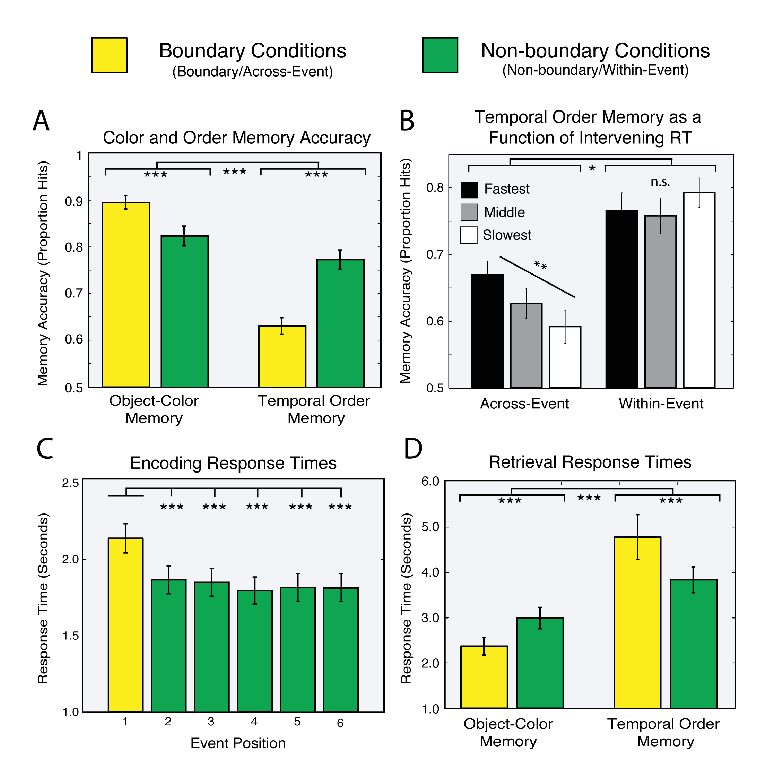
\includegraphics[width=.75\textwidth]{figures/chapter1_figure3.eps}
  \caption[Behavioral Experiment 2 Results]{\textit{Experiment 2 Results.} (A) Memory accuracy is shown as a function of test and condition. (B) Temporal order memory accuracy split into terciles by encoding response time of intervening boundary (for across-event) or non-boundary (for within-event) trial.  (C) Task response times during encoding as a function of event position. (D) Retrieval response times for correct trials as a function of condition and memory test. All error bars represent standard error of the mean across subjects.  *p<.05, **p<.005, ***p<.001. }
  \label{chapter1_figure3}
\end{figure}

\subsubsection{Effect of perceptual boundaries on object-color and
temporal order
memory}\label{effect-of-perceptual-boundaries-on-object-color-and-temporal-order-memory}

Accuracy for object-color memory and temporal order memory was
calculated in two ways: First, we looked at the overall proportion of
correct responses as a function of test condition. Secondly, if the data
varied by confidence, then we separated correct trials by confidence
(HC/LC) and calculated memory accuracy for each condition. Finally, we
assessed whether there was an interaction between boundary/non-boundary
status and memory test type (color/order).

We found that object-color memory accuracy for boundary trials was
significantly better than non-boundary trials {[}\emph{t}(23) = 5.80,
\emph{p} \textless{} .001, Cohen's \emph{d} = 1.96; see Figure 3a{]}.
There was no condition by confidence interaction, so we did not separate
the data by confidence {[}\emph{F}(1,23)=.73,
\emph{p}\textgreater{}.1{]}. These analyses suggest that the event
boundary significantly increased memory for the object-color
association. This result replicates the boundary-related memory
enhancement reported in Experiment 1.

By contrast, temporal order memory was significantly better for the
within-event condition relative to the across-event condition
{[}\emph{t}(23) = 5.37, \emph{p} \textless{} .001, Cohen's \emph{d} =
1.53{]}. There was a significant condition by confidence interaction
{[}\emph{F}(1,23) = 11.01, \emph{p}\textless{}.003, \(\eta^{2}\) =
.33{]}, such that the effect was stronger for HC responses
{[}\emph{t}(23) = 6.008, \emph{p} \textless{} .001, Cohen's \emph{d} =
1.78{]} than LC responses {[}\emph{t}(23) = 2.07, \emph{p} = .05,
Cohen's \emph{d} = .63{]}. Taken together with the data above, this
suggests that the boundaries led to a reduction in associative memory
across events while simultaneously increasing associative binding of
representations at the boundary itself. To directly test for this
interaction, we performed a two-way repeated measures ANOVA and found a
significant test type (color/order) by condition (Boundary/Across-event
and Non-boundary/Within-event) interaction {[}Figure 3a; \emph{F}(1,23)
= 45.39, \emph{p} \textless{} .001, \(\eta^{2}\) = .66{]}. This data
shows that perceptual boundaries improved object-color memory at the
boundary itself, but disrupted temporal order memory for object pairs
that spanned the boundary. Together, these findings suggest a
boundary-related trade-off, where memory for boundary information is
enhanced, perhaps at the cost of across-event associative binding.

\subsubsection{Across-event temporal order memory negatively related to
boundary
processing}\label{across-event-temporal-order-memory-negatively-related-to-boundary-processing}

As a further means for asking whether there is a trade-off between
boundary processing and these different forms of memory, our next
analysis assessed whether response times to boundaries at encoding were
related to later color and order memory. We reasoned that increased
encoding response times to boundary items might reflect greater
attention to the item and color on boundary trials and may, in turn, be
related to the temporal order reductions. Thus, we hypothesized that
longer boundary response times may result in worse order memory for
pairs of objects that spanned the boundary. Crucially, however, we
expected no such relationship between non-boundary response times and
temporal order memory for within-event trial pairs.

To test this hypothesis, we first performed a logistic regression using
boundary response times (i.e.~task responses to position 1 items) to
predict across-boundary temporal order accuracy (position 5 and 3
items). We found that there was an inverse relationship, such that
longer boundary response times were related worse temporal order memory
{[}mean slope = -.18, \emph{t}(23) = -2.16, \emph{p} \textless{} .05,
Cohen's \emph{d} = .44{]}. Critically this effect was not present when
we used non-boundary response times (i.e.~task response times to
position 4 items) to predict within-event temporal order memory
(position 2 and 6 items) {[}mean slope = .19, \emph{t}(23) = 1.32,
\emph{p} \textgreater{} .1{]}. Furthermore, a paired t-test revealed
that the regression slope for the boundary condition was significantly
more negative than the non-boundary regression slope {[}\emph{t}(23) =
-2.35, \emph{p} \textless{}. 05, Cohen's \emph{d} = .66{]}, suggesting a
specific relationship where longer boundary response times were related
to worse across-event temporal order memory.

As a second approach to test this hypothesis, we divided boundary
encoding response times into terciles and assessed temporal order memory
separately for each bin. This complementary analysis allowed us a way to
better visualize the data as well as a way to reduce some of the
variance of response times driven by noise. To test whether boundary
(but not non-boundary) response times are related to temporal order
memory, we conducted a two-way repeated measures ANOVA. There was a
significant condition (boundary/non-boundary) by response time tercile
(slowest, middle, fastest) interaction {[}\emph{F}(2,46) = 4.23,
\emph{p} \textless{} .05, \(\eta^{2}\) = .156{]}. This interaction was
driven by the fact that order memory performance was the lowest in the
slowest tercile of response times and was the best in the fastest
tercile of boundary response times {[}Figure 3b; fastest vs.~slowest:
\emph{t}(23) = 3.03; \emph{p} = .005, Cohen's \emph{d} = .88{]}.
Crucially, no effect of response time on order memory for the analogous
intervening trial in the non-boundary condition was evident {[}fastest
vs.~slowest: \emph{t}(23) = -1.20; \emph{p} =.24{]}. That is, the
response time to the item in the 4th event position was not related to
within-event order memory (between the items in the 2nd and 6th event
position). Furthermore, there was a significant linear trend for
across-boundary temporal order memory as a function of boundary response
tercile {[}\emph{F}(1,23) = 9.23, \emph{p} = .006, \(\eta^{2}\) =
.286{]} that was not present for the analogous within-event condition
{[}\emph{F}(1,23) = 1.44, \emph{p} \textgreater{}.1{]}, and there was a
significant condition (boundary vs.~non-boundary) by tercile (slowest,
middle fastest) interaction in the linear term {[}\emph{F}(2,46) = 4.23,
\emph{p} \textless{} .05, \(\eta^{2}\) = .25{]}, suggesting that the
linear trend was specific to the across-boundary condition. These data
support the notion that event boundaries disrupt temporal order memory
and provide evidence that response time variability on boundary trials
is related to the outcome of temporal order memory for the trials that
span the boundary. In contrast, response times to an intervening item
within events do not appear to be related to temporal order memory.

We then ran a separate control analysis to test whether this
relationship between boundary response time and temporal order memory
was specific to the boundary item. It's possible that rather than
temporal order memory being specifically related to processing at the
boundary, memory could vary as a function of the overall speed of
processing across the sequence of items. In other words, order memory
could vary as a function of the mean encoding response time across the
tested items (i.e.~all trials that intervened the later tested items),
rather than to the boundary item specifically. To address this, we
averaged encoding response times across sequences of items that crossed
a boundary, where the flanking items of the sequence were boundary
temporal order test pairs. Importantly, we excluded the boundary
response itself, but included the other intervening items. Then, we
again sorted the data into terciles, and computed temporal order memory
separately for each response time bin. If the relationship between the
speed of boundary response time and temporal order memory were specific
to the processing of the boundary item, then the average response time
across the sequence would not predict temporal order memory. However, if
temporal order memory co-varied with the mean response time across a
sequence, than we would expect a pattern similar to the previous
analysis, where longer response times predicted worse order memory
performance. A one-way ANOVA revealed that mean response time for
sequences of trials that crossed an event boundary was not predictive of
temporal order memory {[}\emph{F}(2,46{]}=.52, \emph{p} \textgreater{}.
1{]}, providing further evidence that boundary processing is
specifically related to across-trial associative encoding. Together with
the accuracy data described above, these results argue for a trade-off
between boundary processing and across-event mnemonic binding.

\subsubsection{Encoding response times}\label{encoding-response-times-1}

Replicating the results from Experiment 1, we see that response times
during encoding varied as a function of within-event position {[}Figure
3c; \emph{F}(5,115) = 50.63, \emph{p} \textless{} .001, \(\eta^{2}\) =
.69{]}, and a planned contrast revealed that task responses on boundary
items (position 1) were significantly slower than non-boundary items
{[}position 2-6; \emph{t}(23) = 8.07, \emph{p} \textless{} .001, Cohen's
\emph{d} = 2.36{]}. Follow up t-tests show that each pairwise difference
is significant {[}1 vs.~2-6, \emph{p}'s \textless{} .001{]}.

\subsubsection{Retrieval response times}\label{retrieval-response-times}

Finally, we compared response times for correct color and order memory
retrieval as a function of condition. The goal of this analysis was to
see whether the relative increase in memory performance we observed in
the previous color and order accuracy analyses (i.e.~Figure 3a) was also
accompanied by a speeding of the retrieval response. To test whether the
pattern of response times across conditions was dependent on confidence,
we conducted a repeated measures two-way ANOVA and assessed the
condition by confidence interaction. The interaction was not significant
for order {[}\emph{F}(1,23) = .15, p\textgreater{}.1{]} or color
{[}\emph{F}(1,23) = .28, \emph{p} \textgreater{} .1{]}, so we collapsed
across confidence. We found that response times for correct color memory
retrieval trials were significantly faster for B trials relative to NB
trials {[}\emph{t}(23) = 7.3, \emph{p} \textless{} .001, Cohen's
\emph{d} = 2.45; Figure 3d{]}. On the order memory test, better
performance on the within-event trials was accompanied by faster
response times relative to the across-event trials {[}\emph{t}(23) =
3.91, \emph{p} \textless{} .001, Cohen's \emph{d} = 2.28{]}.
Additionally, a two-way repeated measures ANOVA revealed a significant
memory test by condition interaction {[}\emph{F}(1,23) = 32.77, \emph{p}
\textless{} .001, \(\eta^{2}\) = .588{]}. In sum, mnemonic
representations in conditions with better memory (boundary object color
and within-event temporal order) were also accessed more quickly at
retrieval.

\subsection{Discussion}\label{discussion-1}

The results of the Experiment 2 provide evidence that while associative
memory was enhanced for representations presented at perceptual
boundaries, these boundaries resulted in a decrease in temporal order
memory for items studied in adjacent events (Figure 3a). The reduction
in temporal order memory observed is consistent with previous work
showing event boundary-related reductions in cued recall for narrative
stimuli \autocite{ezzyat_what_2011}, as well as an influence of
boundaries on temporal memory for visual images
\autocites{dubrow_influence_2013}{ezzyat_similarity_2014}.
Interestingly, our temporal order memory effects emerged using a simple
color manipulation, demonstrating that boundary-related temporal memory
disruptions can result from simple changes in a perceptual feature of an
event. Moreover, we found that slower boundary encoding response times
were associated with worse temporal order memory for objects spanning
those boundaries. In other words, the larger the magnitude of the
`boundary effect' (as indexed by response time), the worse the temporal
order memory for pairs of objects that spanned the boundary. The current
data supports previous work by replicating the boundary-related
reduction of across-event temporal order memory and importantly extends
it to suggest a trade-off between boundary processing itself and
across-event order memory. In other words, this data highlights the idea
that orienting to something salient in the environment comes at the cost
of the ongoing maintenance of items over time.

Our finding of relatively better temporal order memory for within-event
items as compared to across-event items is also consistent with buffer
models of episodic memory
\autocites{atkinson_human_1968}{lehman_global_2009}{lehman_buffer_2013}{raaijmakers_search_1981}.
\textcite{lehman_buffer_2013} 's buffer model hypothesizes that during
encoding, a buffer process exists that can maintain or drop information
depending upon the goals of the subject or the demands of the task.
Items and contexts that are maintained in the buffer become
associatively linked, while information experienced in different buffers
does not become as strongly associated. In our task, we hypothesize that
items encountered in the same color are maintained in the same buffer
whereas a switch in color (i.e.~perceptual event boundary) may serve as
a cue for the brain to flush the contents of the current buffer, thus
creating an associative disconnect between items studied in different
contexts. Thus, one possible explanation for our observed difference
between within and across event temporal order memory is that items
encountered within the same event occupy the same buffer and thus are
more strongly bound to each other than items encountered in different
events (i.e.~distinct buffers).

Buffer models of episodic memory have been quite successful at
accounting for patterns in episodic memory, particularly in studies with
an intentional forgetting component \autocite{lehman_buffer_2013}.
Typically in these studies, at the end of an encoding list, subjects are
instructed on whether or not to forget the previously studied list. The
model predicts that the cue to forget causes a flushing of the
previously studied items from the buffer (a buffer operation the authors
call ``compartmentalization''). One major difference between our study
and these prior studies is that we do not explicitly instruct
participants to forget between events. In fact, we encourage
participants to bind together items irrespective of the background
color. Thus, a possible interpretation of our findings is that
perceptual event boundaries serve as a bottom-up cue that triggers the
brain to remove the contents of the current buffer. Thus,
compartmentalization may occur spontaneously if there is sufficient
perceptual change in the environment. Future work should be conducted to
characterize whether the nature of the task (i.e.~top-down vs.~bottom-up
compartmentalization) has differential consequences for the organization
of events in episodic memory.

Finally, the memory `trade-offs' reported here can be contrasted with a
body of literature investigating block-level or instruction-level
trade-offs in item vs.~associative in formation in memory
\autocites{einstein_levels_1980}{gronlund_time_1989}{hockley_tests_1996}{hunt_relational_1981}{sharps_relational_1992}.
In this literature, the overarching theme is that when item encoding is
prioritized over associative or relational encoding, item memory
benefits and associative memory suffers. In contrast, when associative
memory is prioritized, there is a benefit for associative memory but
interestingly, item memory remains intact. In the current work, we show
that at event boundaries, when attention is presumably redirected from
item-item associative processing to more local item-context processing,
across-event temporal order memory suffers, while boundary item-context
memory is enhanced. To coalesce these findings, it appears that
regardless of whether the manipulation is top-down and extended in time
(such as an instructional manipulation) or bottom-up and dynamic (such
as a perceptual event boundary in the current design), attention to
`in-the-moment' representations trades off with more temporally extended
relational encoding (i.e.~focusing on item-item relationships). Thus, in
contrast to previous work, the results reported in the current study
highlight the temporally dynamic nature of item and relational tradeoffs
during episodic memory encoding.

\section{Experiment 3: Perceptual boundaries impose structure on verbal
free
recall}\label{experiment-3-perceptual-boundaries-impose-structure-on-verbal-free-recall}

\subsection{Introduction}\label{introduction-2}

So far, we've provided evidence that perceptual boundaries enhance
boundary-related associative memory, while simultaneously reducing
across-event temporal order memory, and that the magnitude of the
boundary effect is predictive of the cost in temporal order memory. One
intuitive explanation for this pattern of results is that when
encountering a perceptual boundary, there is a shift in attention to the
processing of the novel color information, which trades off with the
integration of the previous item representation (i.e.~the pre-boundary
trial) and the current (boundary) trial. We reasoned that if
within-event item representations are more strongly integrated than
items that span a boundary, then one might expect within-event items may
be represented more similarly in memory. If asked to recall the items,
this could lead to a greater likelihood of sequentially recalling
within-event items relative to across event items. Thus, in Experiment
3, we tested the hypothesis that the likelihood of making a local
forward transition (e.g.~n+1, n+2, n+3) from boundary items to other
within-event items would be greater than the likelihood of a local
forward transition from pre-boundary items, where forward transitions
would be to items in a new event.

To test this hypothesis, we employed a modified version of the encoding
paradigm used in Experiments 1 and 2 that was optimized to test memory
using verbal free recall (see Design for details). In this experiment,
participants encoded lists of visual objects embedded in a colored frame
with an accompanying verbal label, and after a short distractor task
were instructed to verbally recall as many items as possible.
Critically, like the previous experiments, the studied objects were
embedded on a colored frame that periodically changed in color.

\subsection{Methods}\label{methods-2}

\subsubsection{Participants}\label{participants-2}

Participants were 24 individuals (ages 18-35) recruited from New York
University and the greater New York Metropolitan Area. All participants
gave informed written consent in accordance with the University
Committee on Activities Involving Human Subjects (ACAIHS) and
participated in exchange for monetary compensation. One person was
excluded for chance color memory performance, leaving 23 participants
for all analyses.

\subsubsection{Materials}\label{materials-2}

For this experiment, we used a subset of the objects (totaling 384
grey-scale objects) used in Experiments 1 and 2. We also included a
written label displayed below each presented object to encourage
participants to use the same label during verbal recall. Each list was
designed to have minimal conceptual overlap, to minimize confusion
during free recall scoring as well as semantic clustering at retrieval.

\subsubsection{Design}\label{design}

In this experiment, participants studied lists of 24 objects (along with
a written label) embedded in a colored frame that changed to a new color
after every 4 trials. Like the previous experiments, there were 6
`events' and 5 `event boundaries' per list. We chose to present 24 items
per list rather than 36 (as in Experiment 1 and 2) due to pilot data
suggesting poor free recall performance when longer study lists were
used. Additionally, we reduced event length from 6 to 4 items to ensure
adequate power for the free recall analyses (i.e.~to have sufficient
boundary trials). Like Experiments 1 and 2, trials that were studied
concurrently with a color change are considered ``boundary'' trials and
objects studied in the other event positions (2-4) are called
``non-boundary'' trials.

\subsubsection{Procedures}\label{procedures}

For each list (12 total), participants encoded 24 object-color pairs.
Participants were instructed to imagine the object in the color of the
frame and make a pleasantness judgment on the object/color combination.
After each study list, participants completed a distractor task in which
they were asked to indicate whether arithmetic problems were correct or
incorrect (e.g. ``5+4+2=11?''). The numbers 1-6 were used for the
arithmetic problems, and the probability of the answer being correct was
50\%. Each problem was presented for 3 seconds for a total of 10
problems during each distractor period (30 seconds). They were also
given immediate feedback to encourage engagement. Following the
distractor task, participants were presented with a screen prompting
them to say ``Next Block'' and then verbally recall as many words as
they could. They were given a minimum of 90 seconds and told to use more
time if they felt they could recall more words. A schematic of a block
of the experiment is displayed in Figure 4a.

Audio was recorded throughout the entire session. Unclear responses were
excluded from the analysis. Synonyms to words that were actually studied
were not considered correct responses. For example, if the correct
response was ``panther'' and the subject reported ``leopard'', this
would not be considered a correct response. However, partial answers
were counted as correct. For example, if the correct response was ``toy
train'' and the subject responded ``train'', it would be marked as
correct. The total number of excluded trials (combining across synonyms,
unclear responses and prior list intrusions) was small (3.7\%). Analysis
of the free recall audio files was performed by one author and one
research assistant using Penn TotalRecall,
(http://memory.psych.upenn.edu/TotalRecall). Using this program, the
onset and serial recall order of each retrieved object was recorded.
Crucially, scorers were blind to the encoding condition to which each
object belonged.

After each free recall period, participants were given an object-color
memory task following the same protocol as Experiments 1 and 2. The
object-color memory test was self-paced. For this experiment, we tested
color memory for all 24 studied items in the list. Across the entire
experiment, there were a total of 36 color memory test trials for each
condition (event positions: 1-4).

\subsection{Results}\label{results-2}

\begin{figure}
  \centering
  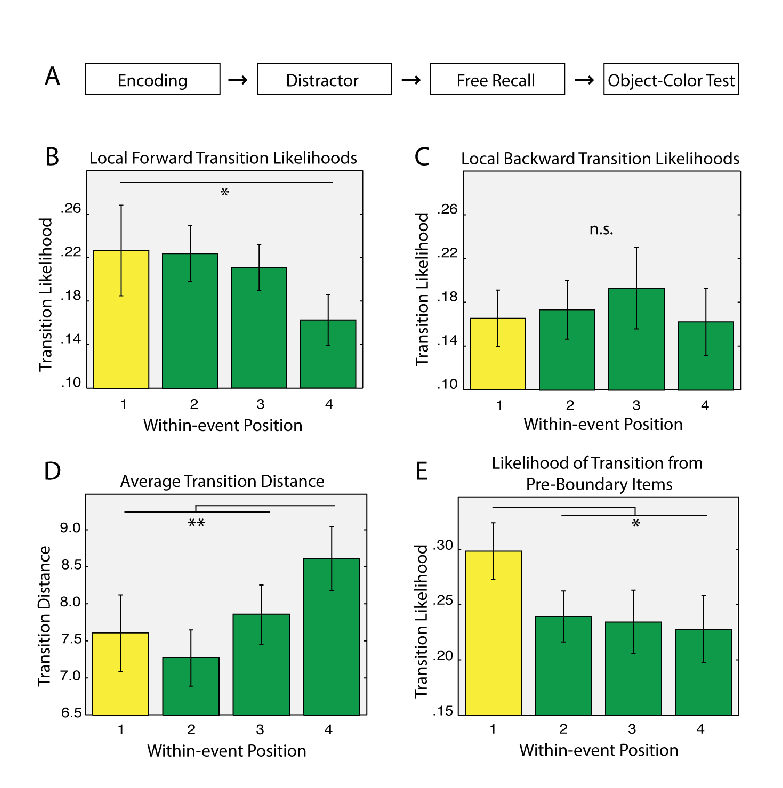
\includegraphics[width=.75\textwidth]{figures/chapter1_figure4.eps}
  \caption[Behavioral Experiment 3 Results]{\textit{Experiment 3 Results.} (A) Task schematic. (B) Local forward (sum of n+1, n+2, n+3) transition likelihood as a function of within-event position. (C) Local backward (sum of n-1, n-2, n-3) transition likelihood as a function of within-event position. (D) Average transition distance as a function of within-event position.  (E) Likelihood of transition from pre-boundary items as a function of within-event position.  *p<.05, **p<.005.}
  \label{chapter1_figure4}
\end{figure}

\subsubsection{Free recall performance}\label{free-recall-performance}

\emph{Overall performance.} Participants recalled an average of 31.30\%
(\(\sigma\) = 12.6\%) of the items presented for each list (or 7.51 out
of 24 items per list). As expected, free recall varied as a function of
serial position of the list {[}\emph{F}(23,506) = 6.82, \emph{p}
\textless{} .001, \(\eta^{2}\) = .237, Supplemental Fig. 1{]}, where
items at the beginning and the end of the list were more likely to be
recalled than items in the middle of the list
\autocite{murdock_serial_1962}. We also computed free recall performance
as a function of event position within an event, but did not observe an
effect {[}\emph{F}(3,66) = .96, \emph{p} \textgreater{} .1{]}, meaning
that all event positions 1-4 were equally likely to be recalled. We
discuss the implication of this finding in more detail in the general
discussion.

Then, we computed the mean lag-conditional response probability
(lag-CRP) curve (Supplemental Figure 2; see
\autocite{kahana_associative_1996}) which showed that, given free recall
of an item, participants were most likely to make free recall
transitions to items in neighboring list positions, consistent with
previous reports
\autocites{howard_distributed_2002}{kahana_associative_1996}.

\emph{Local transition probabilities in free recall.} To measure the
influence of perceptual event boundaries on free recall, our next
analysis focused on local transition probabilities. That is, given the
recall of item n, what is the likelihood of the next item recalled being
locally forward (i.e.~n+1, n+2, or n+3) or locally backward (i.e.~n-1,
n-2, or n-3)?. First, we focused on local forward transitions up to a
lag of three because for boundary items, local forward transitions would
be to other within-event items whereas for pre-boundary items
(i.e.~position 4 items), local forward transitions would be to items in
the next event. We predicted that there would be a greater likelihood of
local forward transitions from boundary items as compared to
pre-boundary items due to the fact that local forward transitions from
boundary items would be to other within-event items. To test this
prediction, for each within-event position, we computed the likelihood
of a local forward transition (i.e.~the sum of the number of transitions
from n to n+1, n+2, and n+3) divided by the number of transitions to all
other items. This resulted in a measure representing the proportion of
the time participants made a local forward transition relative to all
other transitions to items elsewhere in the list. Critically, there were
no differences in the total number of items recalled for each
within-event position (see Free Recall Performance Section) and thus,
the above analysis is only sensitive to the order of free recall, rather
than the total number of items recalled. The results of this analysis
are plotted in Figure 4b. Consistent with our hypothesis, we found that
local forward transitions from boundary and pre-boundary items were
significantly different from each other {[}\emph{t}(22) = 1.88, \emph{p}
\textless{} .05, one-tailed, Cohen's \emph{d} = .71{]}, where relatively
more local forward transitions were made from boundary items. This data
is consistent with the idea that perceptual event boundaries influence
the structure of free recall behavior.

Next, we tested the idea that local backward transitions from
pre-boundary items might be relatively more likely than local backwards
transitions from boundary items because for pre-boundary items, local
backwards transitions were to other within-event items. We performed the
same analysis as described above, but now for only local backwards
transitions as a function of within-event position (Figure 4c).
Interestingly, we did not observe the predicted effect that local
backward transitions would be relatively more likely for pre-boundary
items as compared to boundary items {[}\emph{t}(22) = .10, \emph{p}
\textgreater{} .9{]}. To summarize, while local forward transitions were
more likely from boundary relative to pre-boundary items, there was no
difference in the likelihood of backward transitions.

\emph{Distal transition probabilities in free recall.} The intriguing
result that there were no differences in backward transition
probabilities led us to the follow question: If participants are not
transitioning from pre-boundary items to other within-event items
(i.e.~local backward transitions), to which items are they are more
likely to transition? We reasoned that if local forward transitions from
pre-boundary items are relatively unlikely (as compared to boundary
items) and there were no differences in local backward transitions, then
transitions from pre-boundary items must be to more distal items in the
list. To quantify this, we computed the average transition distance as a
function of position (Figure 4d). That is, given the recall of item n,
what is the average lag of the next recalled item? For this analysis,
our hypothesis was that transitions from pre-boundary items would be to
more distal items relative to all other within-event positions. Put
another way, when one recalls the last item in an event, we predicted
that they would be relatively more likely to transition to a distal
item. To test this hypothesis, we computed a contrast of the average
transition distance from pre-boundary items relative to the other
within-event positions. The analysis revealed that the average
transition distance from pre-boundary items was significantly more
distal than the average transition distance from other within-event
positions {[}\emph{t}(22) = 2.63, \emph{p} \textless{} .05, Cohen's
\emph{d} = .48{]}. Furthermore, the direct comparison of average
transition distance from pre-boundary and boundary items revealed that
pre-boundary transitions are significantly more distal than boundary
transitions {[}\emph{t}(22) = 2.55, \emph{p} \textless{} .05, Cohen's
\emph{d} = .39{]}. Thus, compared to other within-event positions, free
recall transitions from pre-boundary trials are to relatively more
distal items providing further support for the idea that perceptual
event boundaries influence the structure of free recall behavior.

\emph{Transitions from pre-boundary items.} Our last free recall
analysis was designed to test the idea that transitions from
pre-boundary items would be disproportionately more likely to boundary
items relative to items in other within-event positions. We predicted
that given the recall of the last item in an event (and thus terminating
the recall of a particular episode), one might initiate a memory search
process in an attempt to recall additional items. If boundary items
somehow `stand out' in memory
\autocites{radvansky_across_2012}{zacks_event_2007}, then the likelihood
of transitioning to a boundary item given the recall of a pre-boundary
item may be relatively higher than transitioning to other within-event
positions. In this way, boundary items may serve as a `gateway' into an
episodic event. To test this prediction, we computed the conditional
likelihood of transitioning to each within-event position given the
recall of a pre-boundary item (Figure 4e). A contrast of pre-boundary
transitions to boundary items relative to items in other positions
suggests that following the recall of a pre-boundary item, boundary
items are most likely to be recalled next {[}\emph{t}(22) = 1.89,
\emph{p} \textless{} .05, one-tailed, Cohen's \emph{d} = .79{]}. The
direct comparison of pre-boundary transitions to boundary items
vs.~pre-boundary items showed a significant trend {[}\emph{t}(22) =
1.59, \emph{p} = .063, one-tailed, Cohen's \emph{d} = .52{]}. One
potential issue with the analysis described above is that the effect
could be driven solely by local forward transitions (i.e.~a temporal
contiguity effect). To rule out this explanation, we performed the
analysis again, now removing all local transitions (n +/- 1, 2 or 3).
When analyzing only transitions from pre-boundary items to other distal
items (greater than 3 positions away), the effect remained
{[}\emph{t}(22) = 1.73, \emph{p} \textless{} .05, one-tailed, Cohen's
\emph{d} = .60{]}. Thus, consistent with our prediction, following the
recall of the last item in an event, distal boundary items are
significantly more likely to be recalled next (as compared to other
within event positions). Together with the free recall analyses
described above, these data support the idea that perceptual boundaries
introduce structure into free recall behavior.

\subsubsection{Color memory performance}\label{color-memory-performance}

Analysis of variance revealed a trend for color memory to vary as a
function of within-event position {[}\emph{F}(3,66) = 2.57, \emph{p} =
.06, \(\eta^{2}\) = .11{]}. A planned contrast demonstrated object-color
memory was better for boundary trials than non-boundary trials
{[}\emph{t}(22) = 2.67, \emph{p} = .01, Cohen's \emph{d} = .80{]}.
Post-hoc pairwise t-tests revealed that memory was significantly better
for boundary trials than all non-boundary trials {[}\emph{p}'s
\textless{} .05{]} with no other significant differences. The
interaction between confidence and condition was not significant. Note
that in this experiment we replicate Experiments 1 and 2 show that
boundary object-color memory accuracy was better than non-boundary
memory. While the effect was modest in this version of the paradigm,
together with the color memory enhancements observed in both Experiments
1 and 2, these results provide consistent evidence for boundary-related
memory enhancements.

Response times for correct color memory retrieval trials also varied as
a function of within-event position {[}\emph{F}(3,66) = 10.29, \emph{p}
\textless{} .001, \(\eta^{2}\) = .319{]}. A planned contrast between
boundary and non-boundary color retrieval RTs revealed that boundary RTs
were significantly faster than non-boundary RTs {[}\emph{t}(22) = -4.24,
\emph{p} \textless{} .001, Cohen's \emph{d} = 1.26{]}. Post-hoc tests
showed that color retrieval RTs were significantly faster for boundary
trials compared to all non-boundary trials {[}\emph{p}'s \textless{}
.05{]}. There was no significant interaction between condition and
confidence, so these analyses were performed on data collapsed across
condition.

\subsubsection{Encoding response times}\label{encoding-response-times-2}

There was a significant effect of event position on encoding response
times {[}\emph{F}(3,66) = 28.90, \emph{p} \textless{} .001, \(\eta^{2}\)
= .57{]}. A planned contrast reveals that boundary response times were
significantly slower than non-boundary {[}\emph{t}(22) = 6.72, \emph{p}
\textless{} .001, Cohen's \emph{d} = 2.04{]}. Pairwise t-tests revealed
that boundary encoding response times were significantly slower than all
non-boundary trials {[}event positions 2-4, \emph{p}'s
\textless{}.001{]} and there were no other differences. This finding
replicates Experiments 1 and 2 and extends it to include shorter events
(four as compared with six items in Experiments 1 and 2).

\subsubsection{Math accuracy}\label{math-accuracy}

Accuracy on the math task was high (\(\mu\) = .89, \(\sigma\) = .08) and
all participants performed statistically above chance.

\subsection{Discussion}\label{discussion-2}

In the current experiment, we aimed to examine whether and how free
recall organization was influenced by perceptual event boundaries.
Overall, we found that transition likelihoods varied as a function of
within-event position (Figure 4). First, our results suggest that local
forward transitions were significantly more likely from boundary items
as compared to pre-boundary items whereas there were no differences
between conditions for local backward transitions (Figure 4b, c).
Second, we found that transitions from pre-boundary were on average to
more distal items than transitions from other within-event positions.
Lastly, transitions from pre-boundary items were most likely to be to
boundary items as compared to other within-event positions. These
findings argue that perceptual event boundaries influence the structure
of free recall behavior.

Our finding that local forward transitions (n+1, n+2, n+3) were more
likely from boundary items than from pre-boundary items is consistent
with the idea that items encountered in the same event are more strongly
associated to each other than items in distinct events. For boundary
items, forward local transitions were all to other within event items,
whereas for pre-boundary items local forward transitions were all to
items in the neighboring event. This result is in line with temporal
context models of memory
\autocites{howard_distributed_2002}{manning_oscillatory_2011}{polyn_category-specific_2005}{polyn_context_2009},
that propose that during the study of a list of stimuli, items are bound
to a slowly-changing representation of context. Although the particular
features (e.g.~semantic, source, temporal) that are included in the
context representation vary according to the specific model, all
retrieved context models propose that when an item is recalled from
memory, the context representation is reinstated and used to guide the
retrieval process. Because the context representations of neighboring
items are most similar, this leads to free recall transitions between
neighboring items, and the overall lag-CRP pattern. Our data are in line
with such a retrieval interpretation to the extent that the perceptual
details associated with each item are also reinstated during recall.
Thus, reinstatement of the color associated with an object may make it
more likely that participants will recall other objects encoded with the
same color.

In a previous study, \autocite{polyn_context_2009} found that when
freely recalling a short list of 12 words that included one task switch
at the halfway point in the list, participants tended to cluster their
recall responses by items that shared an encoding task. That is, more
free recall transitions were made between words that were encoded using
the same task as compared to words encoded under two different tasks.
Our results are consistent with that result and extend it to suggest
that the change in a perceptual feature during experience is sufficient
to impose structure in the free recall of events. While Polyn and
colleagues focused their analyses on the effect of task boundaries on
the likelihood of within- vs.~across-event transitions (irrespective of
the list position of the item), we specifically asked whether items that
flanked a perceptual boundary would show a within-event bias. This
analytic approach allowed us to determine precisely how boundaries
modulate the likelihood of within-event recall transitions.

Interestingly, while we found that local forward transitions are
significantly more likely from boundary items relative to pre-boundary
items, we found no difference between the two conditions in local
backwards transitions. If shared context results in stronger associative
binding between items in the same event, one might expect local
backwards transitions to be relatively greater for pre-boundary items
compared to other within-event positions, since local backwards
transitions would be to other within-event items. While we note that the
aforementioned result is a null finding (and therefore not directly
interpretable), we can offer a few speculations as to why we might not
expect to see an effect. Previous studies suggest that free recall is
reliably bias in the forward direction
\autocites{kahana_associative_1996}{howard_distributed_2002} and
backwards transitions are relatively more rare. We see this pattern in
our data as well (Figure 4b, 4c; Supp Figure 2). Thus, it's possible
that perceptual boundaries exert a substantially stronger effect on
forward transition probabilities. An alternative explanation is that our
experimental design was not sensitive enough to detect the effect of
boundaries on backward transitions (e.g., lists too long, events too
short or boundaries not strong enough). Nonetheless, the fact that that
we do observe a greater likelihood of local forward transitions from
boundary items as compared to pre-boundary items is evidence that
perceptual boundaries do indeed shape free recall behavior.

A second notable observation from this experiment was that the average
transition distance from pre-boundary items was significantly further
than from boundary items. On other words, given the successful recall of
a pre-boundary item, participants were more likely to next recall a more
distal item in the list. One possible explanation for this finding is
that perceptual event boundaries result in a weak associative link
between a pre-boundary item and its neighboring boundary item
\autocites{dubrow_influence_2013}{ezzyat_what_2011}. Because of this
weak associative link, after the successful recall of a pre-boundary
item, a memory search process might be initiated and as a consequence,
more distal item may be subsequently recalled. This finding is
consistent with the idea that event boundaries disrupt associative
binding between items and suggest that transitions following the recall
of the last item in an event are on average more distal than transitions
fro other within-event positions.

Another interesting finding from this experiment was that following the
successful recall of a pre-boundary item, the next item recalled is most
likely to be a boundary item. Given that pre-boundary items are
neighbored by boundary items and that participants generally tend to
transition forward in free recall, this may not seem entirely
surprising. However, this effect remains significant after removing
local items from the analysis, suggesting that when one transitions from
a pre-boundary item to a more distal item, it tends to be a boundary
item. An intriguing interpretation of this finding is that event
boundaries may serve as a `gateway' into an episodic event. In other
words, after successfully recalling the end of a previous event and
during a mnemonic search for more items, boundary items might stand out
as entry points into other mnemonic episodes. Consistent with this
interpretation, we found that on average transitions from pre-boundary
items were more distal than from other positions and out of those distal
transitions, transitions to boundary items were most probable. While the
`gateway' idea is certainly attractive, future studies will be necessary
to determine if this is the most likely explanation for this pattern of
results.

Finally, event segmentation theory suggests that items encountered at
event boundaries may be more memorable than items encountered elsewhere
in an event, possibly due to increased attention at boundaries
\autocites{radvansky_across_2012}{zacks_event_2007}. All three
experiments are consistent with this idea by showing that object-color
memory is better at event boundaries than at other within-event
positions. Interestingly, however, in Experiment 3 we did not observe an
overall increase in free recall of boundary items, as one might have
predicted from EST. While we hesitate to over interpret this null
finding, we can offer some speculation to why we observed this effect.
Rather than boundaries generally boosting memory for boundary
information, boundaries may selectively increase associative binding
between a boundary item and its context. A mechanism of this nature
would predict greater object-color associative memory, but not
necessarily better encoding of boundary items alone. Alternatively,
perceptual boundaries may generally enhance encoding, but our study may
not have been sensitive enough to detect it. Future work will be
necessary to disentangle whether event boundaries differentially
influence item memory vs.~item-context associative binding.

\section{General Discussion}\label{general-discussion}

The studies presented here demonstrate that perceptual boundaries
influence the organization of events stored in long-term memory. In
Experiment 1, we found that perceptual boundaries enhanced associative
binding between an object and a color background. In Experiment 2, we
show that while boundary-related associative memory was enhanced,
temporal order memory for pairs of items that span a perceptual boundary
was disrupted relative to order memory for within-event item pairs.
Furthermore, the magnitude of the boundary effect (i.e.~the response
time to the boundary) predicted the cost in temporal order memory
suggesting a trade-off between boundary processing and across-event
temporal order memory. Finally, in Experiment 3, we found that
participants exhibited recall behavior that was structured by perceptual
event boundaries. Taken together, this work provides compelling evidence
that perceptual boundaries have a lasting influence on the structure of
our memories.

These results add to a growing body of literature characterizing the
influence of event segmentation on long-term memory
\autocites{boltz_temporal_1992}{dubrow_influence_2013}{ezzyat_what_2011}{ezzyat_similarity_2014}{newtson_perceptual_1976}{schwan_cognitive_2004}{zacks_event_2006}.
Previous studies using naturalistic stimuli have provided data
consistent with the idea that information experienced at event
boundaries is better encoded in memory
\autocites{boltz_temporal_1992}{newtson_perceptual_1976}{schwan_cognitive_2004}.
However, there is some concern that these effects could be explained by
differences in the amount of diagnostic information between conditions;
that is, if boundary test items provide a better `summary' of a
particular event than non-boundary test items, one might expect higher
boundary memory that is not driven by event segmentation processes, per
se. By contrast, in the current study, we carefully matched the boundary
and non-boundary conditions during retrieval, such that the only
difference between the two was their position within an event during
encoding. Thus, the best explanation for the boundary-related memory
enhancement in our study is an influence during encoding of the
perceptual boundary on associative binding (between the object and
color). This effect, which we see across three experiments is consistent
with previous research demonstrating boundary-related memory
enhancements, and confirms that segmentation processes during encoding
lead to better memory for information encoded at event boundaries.

These results are also consistent with studies of contextual novelty
that find that items that are in someway deviant from the local
surroundings show a boost in memory
\autocites{cimbalo_making_1978}{lin_enhanced_2010}{restorff_uber_1933}{swallow_role_2011}{swallow_attentional_2013}{wallace_review_1965}.
Typically, these studies have observed differences in item memory based
on deviance status. The present study is novel in that we find enhanced
item-context associative binding for contextually novel trials
(i.e.~object-color pairs encoded at perceptual event boundaries). While
this distinction may seem subtle, it does not follow that better item
encoding should necessarily entail better item-context associative
memory. For instance, compared to neutral stimuli, emotionally arousing
stimuli show better item memory and worse item-context associative
memory \autocites{bisby_negative_2014}{madan_emotional_2012}.
Furthermore, it is now well established that different neural structures
support the encoding of item information vs.~the binding of an item to
its context
\autocites{davachi_item_2006}{davachi_multiple_2003}{ranganath_dissociable_2004}.
Therefore, it is conceivable that item memory and item-context
associative memory are dissociable memory representations. Future work
should test the relationship between item memory and item-context
associative memory at perceptual boundaries.

In Experiment 2, we found that temporal order memory was relatively
worse for across-event trial pairs relative to within-event trial pairs.
This is consistent with previous results that show that cued recall
\autocite{ezzyat_what_2011} and temporal order memory decisions
\autocite{dubrow_influence_2013} are more accurate for test items that
were from the same `event' compared to those from adjacent `events' --
even though the actual temporal lag was the same in both conditions. The
current study complements these previous results that used more complex
boundaries (e.g.~task/stimulus class switches, narrative temporal
boundaries) by demonstrating that simple perceptual boundaries are
sufficient to induce event segmentation processes that result in better
within-event versus across-event associative memory.

It's worthwhile to note that some theories of recency memory might
predict the opposite pattern of results (see
\textcite{friedman_memory_1993} for review). For instance, if
participants were using an item-strength or contextual overlap retrieval
strategy to recover recency information, a change in context between
items could be beneficial for performance. On the other hand, if
participants are performing recency discrimination by recovering
associative information among a set of items, one might predict that
within-event temporal order memory would be greater than across-event
temporal order memory since shared contextual features can help to bind
items across time. The latter prediction is consistent with our results,
suggesting that rather than a distance-based retrieval strategy,
participants may be relying on retrieving the associative links between
a series of items. Further evidence for this type of retrieval mechanism
comes from a study that found that during a recency discrimination test,
the speed of retrieval for items that intervened the recency test pair
during encoding is facilitated relative to items that did not intervene
the test pair \autocite{dubrow_temporal_2014}. Furthermore, in a related
fMRI experiment, the category of items that intervened the recency test
probes during encoding was ``reactivated'' during successful recency
discrimination \autocite{dubrow_temporal_2014}. Together, these findings
suggest that in at least some cases (i.e.~when the lag between the
tested items is short), recency discrimination can be successfully
performed by recovering the items that intervened the test pair.

Finally, the results from our free recall data (Experiment 3) underscore
the influence of perceptual event boundaries on memory organization.
Namely, we found that perceptual boundaries modulated free recall
transition probabilities: local forward transitions from boundary items
were more likely as compared to local forward transitions from
pre-boundary items (Figure 4). This is likely due to the fact that for
boundary items, local forward transitions were to other within-event
items where as local forward transitions from pre-boundary items were to
items in a different event. This result is consistent with previous
studies that find evidence for recall organization according to the
source of the stimuli
\autocites{frost_clustering_1971}{hintzman_memory_1972}{murdock_modality_1969}{nilsson_further_1974}{polyn_task_2009}.
Interestingly, however, we did not find that local backwards transitions
we more likely for pre-boundary items, as one might expect if recall
organization is strongly influenced by source information. However,
since this was a null finding, its interpretation is not entirely
straight-forward as many factors could have influenced the lack of a
finding. Nonetheless, the fact that we see a larger proportion of local
forward transitions from boundary items compared to pre-boundary items
is evidence that perceptual event boundaries structure memory recall
behavior. We also found that transitions from pre-boundary items were
more likely to be to distal items (as compared to transitions from
boundary items). One interpretation of this result is that when a
participant recalls an item that occurred just prior to an event
boundary, the associative link to the next item was severed by the
perceptual boundary, thus prompting a memory search to recall other
items in the list. A mechanism of this nature could lead to selectively
more distal transitions for pre-boundary items relative to other
within-event positions. Lastly, we found that following the successful
recall of a pre-boundary item, boundary items were most likely to be
recalled next. This was evident for local transitions as well as distal
transitions. One explanation for this pattern of results is that
following the recall of the end of an event, participants may initiate a
memory search process in an effort to recover additional list items. If
boundary items `stand out' in memory due to better overall encoding or
better item-context binding, then the likely of a boundary transition
would be greater than the likelihood of transitioning to other list
positions. This last preliminary data point is consistent with the idea
that event boundaries may act as `gateways' into an episodic events.
That is, during free recall, boundaries may stand out as entry points
into an episodic memory and facilitate the retrieval of additional
within-event information.

\section{Conclusions}\label{conclusions}

Together, Experiments 1 and 2 suggest that while perceptual boundaries
may enhance some forms of memory (i.e.~object-color associative memory),
this comes at the cost of reduced across-event associative memory
(temporal order memory). In other words, shifting one's attention to a
novel stimulus in the environment trades off with the ongoing
maintenance and integration of representations into an event model, and
this causes a disruption in the associative binding of items encountered
across time. Finally, Experiment 3 highlights that perceptual boundaries
influence natural recall behavior and suggests the possibility of a
mechanism where event boundaries may serve as a `gateway' into an
episodic memory. In summary, the findings from all three studies
highlight that organizational processes during encoding influence the
structure of later episodic memories.

\section{Supplemental Figures}\label{supplemental-figures}

\begin{figure}[htbp]
\centering
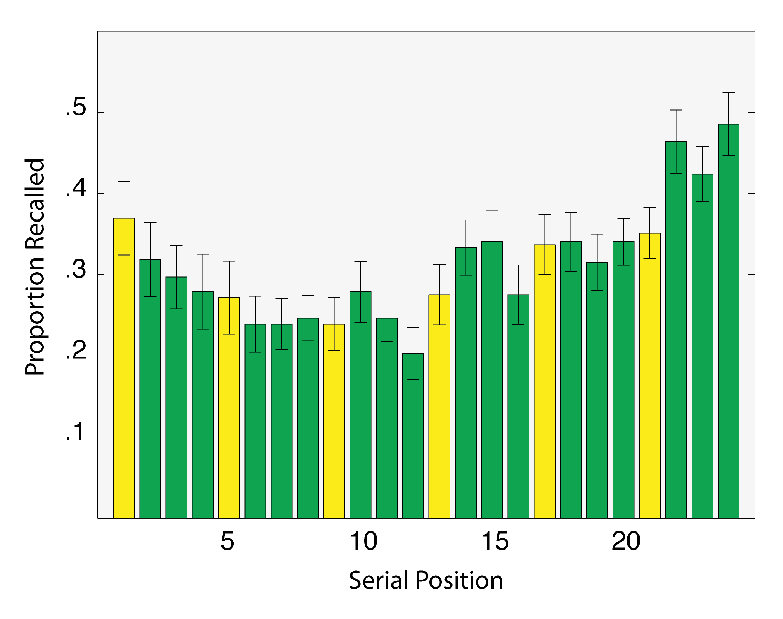
\includegraphics{figures/chapter1_suppfigure1}
\caption{This is the caption}
\end{figure}

\begin{figure}[htbp]
\centering
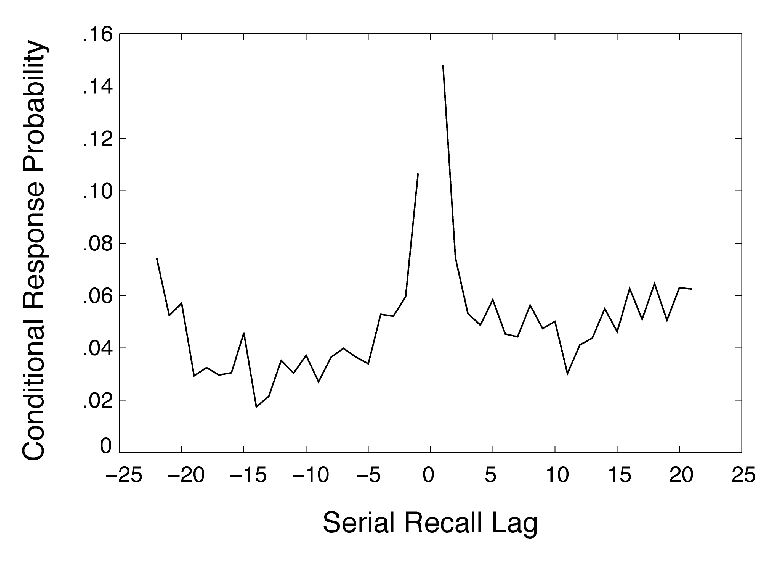
\includegraphics{figures/chapter1_suppfigure2}
\caption{This is the caption}
\end{figure}
